\documentclass{article}
\usepackage{graphicx}
\usepackage[export]{adjustbox}
\usepackage[spanish]{babel}
\usepackage[utf8]{inputenc}
\usepackage[left=2.5cm,
			top=2.5cm,
			right=2.5cm,
			bottom=3cm]{geometry}
\pagenumbering{gobble}

%Materia y maestro
\newcommand{\materia}{\uppercase{Amplificadores Operacionales}}
\newcommand{\maestro}{\uppercase{María De Los Ángeles Fabián Álvarez}}

%Tipo de documento y nombres de tema
\newcommand{\tipoDoc}{\uppercase{}} %TAREA, REPORTE DE LABORATORIO,
\newcommand{\nombreDoc}{\uppercase{Investigación}} 
\newcommand{\docNum}{}
\newcommand{\subNombreDoc}{\uppercase{Características de los circuitos integrados LM324 y TL084}}

%Alumnos y fecha
\newcommand{\alumnos}{\uppercase{GABRIEL AGUILAR LEMUS \\ Jorge Alberto Ochoa López}}
\newcommand{\fecha}{\uppercase{13 de Septiembre de 2017}}

\usepackage[binary-units]{siunitx}
\newcommand{\unidad}[1]{\,\si{#1}}

\begin{document}
	%Cabezal del membrete
	
	\includegraphics[scale=.5, center]{/home/gabriel/LATEX/PortadaOficial/encabezado.png}
	\begin{center}
{
	\huge INSTITUTO TECNOLÓGICO DE MORELIA \\
	\vfill
	\large DIVISIÓN DE ESTUDIOS PROFESIONALES  \\
	\vfill
	\large  DEPARTAMENTO DE INGENIERÍA ELECTRÓNICA \\ 
	\vfill
	\Large \textbf \materia \\
	\vfill
	\textbf{\tipoDoc} \\
	\vfill 
	\LARGE  \textbf{ \nombreDoc  \, \docNum: \\ \subNombreDoc} \\
	\vfill
	\large PRESENTA(N): \\
	\LARGE  \textbf{\alumnos} \\
	\vfill
	\large PROFESORA: \\
	\Large \textbf{\maestro }
}
	\end{center}
	\vfill 
	\begin{flushleft}
		MORELIA, MICHOACÁN \hfill \uppercase{\fecha}
	\end{flushleft}
	\pagebreak
	\section{Integrado TL084}
	Del circuito integrado TL084 se encontraron en la hoja de datos las siguientes magnitudes de las características solicitadas.
	\paragraph{Determinar si el Amp. Op. es rail-to-rail, si no, buscar los valores de saturación.}
	La datasheet indica que los Amp. Op. del circuito integrado no son tipo rail-to-rail dado que no se menciona dicha característica en el listado de características. Además, en la sección 6.5 y 6.6 de la hoja de datos, características eléctricas de la familia de dispositivos TL08xC, TL08xxC, TL08xI, TL08xM y TL084x; se indica el parámetro de máximo voltaje pico de salida alimentando el dispositivo con fuentes simétricas de $V_{CC \pm} = \pm 15 \unidad{V} $. Este parámetro tiene un valor típico de $\pm 12 \unidad{V}$ en los rangos de operación indicados y con una carga mayor o igual a $10 \unidad{k \Omega}$. Estos son los valores de saturación para el dispositivo dadas las condiciones de medición presentadas.
	\paragraph{Determinar si el Amp. Op. puede alimentarse con una sola fuente, ¿valores?.}
	La hoja de datos indica en la sección 6.3, condiciones de operación recomendadas, que los voltajes de alimentación, llamados $V_{CC+}$ y $V_{CC-}$ se encuentren ambos dentro de un mínimo de $5\unidad{V}$ y $-5\unidad{V}$ respectivamente y un máximo de $15\unidad{V}$ y $-15\unidad{V}$ respectivamente. Por lo tanto requiere dos fuentes de alimentación.
	\paragraph{Slew Rate}
	El slew rate típico de esta familia de Amp. Op. es $13 \unidad{V/\mu s}$. En la figura \ref{fig:figura19_tl084} se muestra el circuito de medición de este parámetro que indica la hoja de datos. También se indica que esta medición se realizó en el punto de ganancia unitaria alimentado con $V_{CC \pm} = \pm 15 \unidad{V} $ y a una temperatura de $25 \unidad{^{\circ} C}$.
	
	\begin{figure}[h!]
		\centering
		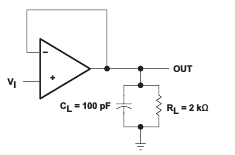
\includegraphics[scale=1]{img/figura19_tl084}
		\caption{Tomado de la hoja de datos. Circuito de medición para el parametro slew rate.}
		\label{fig:figura19_tl084}
	\end{figure}
	\paragraph{CMRR.}
	En la sección 6.5 y 6.6 de la hoja de datos, características eléctricas de la familia de dispositivos TL08xC, TL08xxC, TL08xI, TL08xM y TL084x; se establece la taza de rechazo de modo común con un valor de $86\unidad{dB}$.
	\paragraph{Voltaje de offset.}
	En la sección 6.5 y 6.6 de la hoja de datos, características eléctricas de la familia de dispositivos TL08xC, TL08xxC, TL08xI, TL08xM y TL084x; se establece el valor de voltaje de offset de entrada con valores que se encuentran en el rango de $3$ a $15 \unidad{mV}$.
\end{document}

